 \documentclass{report}

\usepackage{pgfplots}
\pgfplotsset{width=5.5in,compat=1.10}

\begin{document}
 
\begin{center}
\textbf{Graphs}
\end{center}

\begin{flushleft}
\textbf{1. Finding $q_*$}
\end{flushleft}

\begin{flushleft}
We will consider four ways to find $q_*$ = $M^tq_0$ as t $\rightarrow$ $\infty$
\end{flushleft}

%%%%%%%%%%%%%%%%%%%%%%%%%%%%%%%%%%%%%%%%%%%%%%%%%%%%%%%%%%%%%%%%%%%%%%%%%%

\begin{flushleft}
\textbf{A (40 points): Run each method (with t = 1024, $q_0$ = $[1, 0, 0, . . ., 0]^T$ and $t_0$ = 100 when needed) and report the answers.}
\end{flushleft}

\begin{flushleft}
Random Walk = [0.0574, 0.0669, 0.0822, 0.0954, 0.1340, 0.0918, 0.1581, 0.1341, 0.1024, 0.0778]
\end{flushleft}

\begin{flushleft}
Eigen Analysis = [0.0574, 0.0670, 0.0822, 0.0954, 0.1339, 0.0917, 0.1583, 0.1339, 0.1023, 0.0779]
\end{flushleft}

\begin{flushleft}
Matrix Power = [0.0574, 0.0670, 0.0822, 0.0954, 0.1339, 0.0917, 0.1583, 0.1339, 0.1023, 0.0779]
\end{flushleft}

\begin{flushleft}
State Propagation = [0.0574, 0.0670, 0.0822, 0.0954, 0.1339, 0.0917, 0.1583, 0.1339, 0.1023, 0.0779]
\end{flushleft}

%%%%%%%%%%%%%%%%%%%%%%%%%%%%%%%%%%%%%%%%%%%%%%%%%%%%%%%%%%%%%%%%%%%%%%%%%%

\begin{flushleft}
\textbf{B(20points): Re-run the Matrix Power and State Propagation techniques with $q_0$ = $[0.1,0.1,...,0.1]^T$. For what value of t is required to get as close to the true answer as the older initial state?}
\end{flushleft}

\begin{flushleft}
Matrix Power= [0.0574, 0.0669, 0.0822, 0.0954, 0.1340, 0.0918, 0.1581, 0.1341, 0.1024, 0.0778]

$\newline$
So, at t = 85, you get the above, which are close enough
\end{flushleft}

\begin{flushleft}
State Progation= [0.0574, 0.0669, 0.0822, 0.0954, 0.1340, 0.0918, 0.1581, 0.1341, 0.1024, 0.0778]

$\newline$
So, at t = 85, you get the above, which are close enough
\end{flushleft}

\begin{flushleft}
The t we got was 85, but if you want to be a little less accurate then you can get a smaller t, and if you want to be more accurate you get a bigger t, it all depends on how accurate you want to be.
\end{flushleft}

%%%%%%%%%%%%%%%%%%%%%%%%%%%%%%%%%%%%%%%%%%%%%%%%%%%%%%%%%%%%%%%%%%%%%%%%%%

\begin{flushleft}
\textbf{C (24 points): Explain at least one Pro and one Con of each approach. The Pro should explain a situation when it is the best option to use. The Con should explain why another approach may be better for some situation.}
\end{flushleft}

\begin{flushleft}
Matrix Power: If the matrix is of a higher dimensions or t is really big, the matrix multiplication of M * M can get really expensive. Don't use when M is of huge dimension or t is huge, use it otherwise. The short cut of when the t is a power of 2 is not useable if the t is not a power of two, but a great advantage if t is a factor of 2.

$\newline$
State Propagation: If the matrix is of a higher dimensions or t is really big, the M * $q_i$ can get really expensive. Don't use when M is of huge dimension or t is huge, use otherwise. This should be better than Matrix power because its a matrix
multiplied by a vector.

$\newline$
Random Walk: If the matrix M dimensions are huge then this might be a faster approach depending on how you calculate the next step proportional to the probability. This approach is random so it might not be the most accurate, but with
enough runs you should get a really close estimate, but multiply runs will affect performance, so it's a balance. This approach has great performance, but it also lacks the disadvantage that you only have counters and positions instead of the information of the whole matrix. This approach loses a lot of information, if you need that extra information another approach might be better, use otherwise.

$\newline$
Eigen-Analysis: This approach is simple and does not even require a q starting point or a t. Use when you don't have a q starting point or t. This approach is among the simplest to do. This method also loses some of the information of the matrix, if you need that information don't use this method.
\end{flushleft}

%%%%%%%%%%%%%%%%%%%%%%%%%%%%%%%%%%%%%%%%%%%%%%%%%%%%%%%%%%%%%%%%%%%%%%%%%%

\begin{flushleft}
\textbf{D (8 points): Is the Markov chain ergodic? Explain why or why not.}
\end{flushleft}

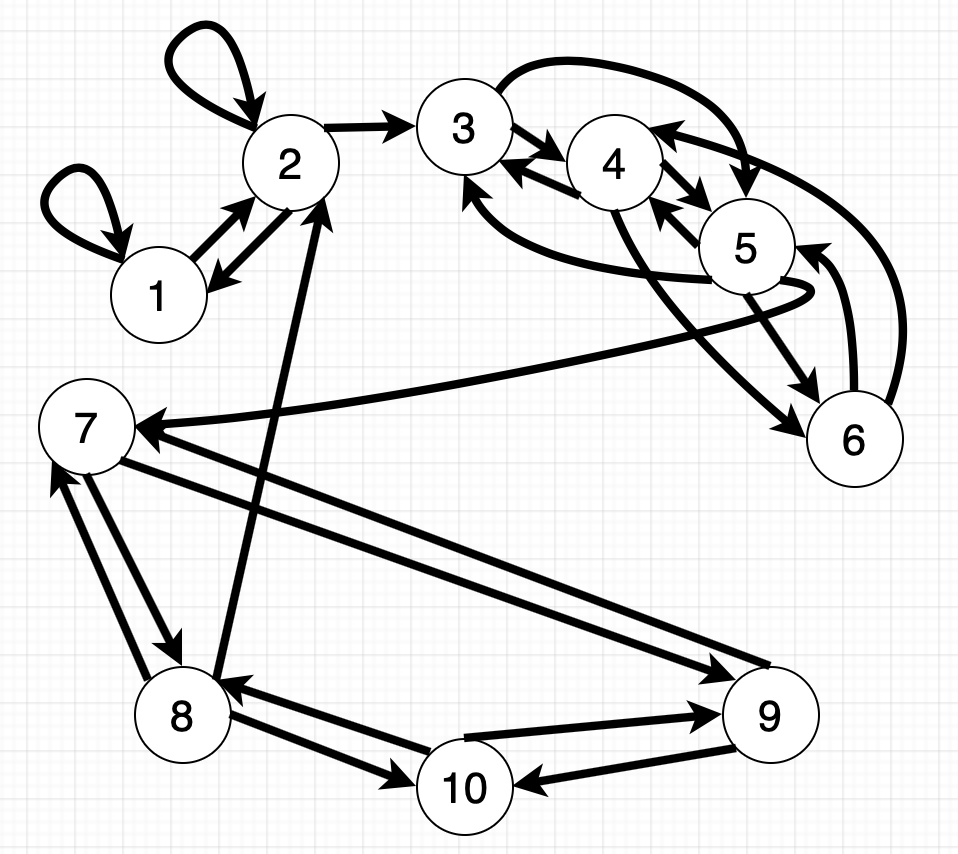
\includegraphics [width = 1 \textwidth] {Graph}

\begin{flushleft}
The Markov Chain is Ergodic because it does not meet any of the following requirements.

1. It is cyclic. This means that it alternates between different sets of states every 2 or 3 or in general p
steps. Here are some example cyclic transition matrices

2. It has absorbing and transient states. (This only happens when the initial graph is directed, so you cannot go backwards on an edge. ) In some Markov chains we can classify V into two class A, T $\subset$ V so that if a random walk leaves some node in T and lands in a state in A, then it never returns to any state in T . In this case, the nodes A are absorbing, and the nodes in T are transient. Here are some examples

3. It is not connected. There are two sets of notes A, B $\subset$ V such that there is no possible way to
transition from any node in A to any node in B. And some examples
\end{flushleft}

%%%%%%%%%%%%%%%%%%%%%%%%%%%%%%%%%%%%%%%%%%%%%%%%%%%%%%%%%%%%%%%%%%%%%%%%%%

\begin{flushleft}
\textbf{E (8 points): Each matrix M row and column represents a node of the graph, label these from 1 to 10 starting from the top and from the left. What nodes can be reached from node 4 in one step, and with what probabilities?}
\end{flushleft}

\begin{flushleft}
[0 0 .3 0 .3 .4 0 0 0 0]
\end{flushleft}

\begin{flushleft}
Node 3 with 30\%, Node 5 with 30\%, and Node 6 with 40\%
\end{flushleft}
 
 \end{document}